\documentclass[a4paper,12pt]{article}

\usepackage[finnish]{babel}
\usepackage[latin1]{inputenc}
\usepackage[dvips]{graphicx}
%\usepackage[T1]{fontenc}
\usepackage{amsmath}

%% parskip pakettin avulla kappaleenvaihdot tehd��n tyhj�ll� rivill�
%% ilman sisennyksi�
\usepackage{parskip}

%% icomma-paketti muuttaa matematiikkamoodin syntaksia niin, ett� pilkku
%% ladotaan tavalliseen tapaan, jos sen j�lkeen on kirjoitettu v�lily�nti,
%% ja desimaalipilkkuna muuten.
\usepackage{icomma}

%% verbatim paketin mukana tulee comment environmentti
\usepackage{verbatim}

%% subfig paketti antaa subfloat komennot useiden kuvien liitt�miseen
%% yhteen figure environmentiin
\usepackage{subfig}

%% caption paketilla voi s��t�� floatien captionien tyyli�
%% hyv�t arvot captionsetupille: margin=10pt,font=small,labelfont=bf
\usepackage{caption}
\captionsetup{margin=1cm,font=small,labelfont=bf}

%% asetetaan listoille labeli
\def\lstlistingname{Listaus}

% t�m� paketti antaa url-komennon
\usepackage{url}

%% listingsutf8 paketti mahdollistaa UTF-8 listausten lataamisen
%\usepackage{listingsutf8}

\begin{document}

% Kansilehti
\begin{titlepage}
\pagestyle{empty}

\begin{tabbing}
AS-74.3135 \` 26.04.2009�\\
Servotekniikka
\end{tabbing}

\vspace*{7cm}
\begin{center}
\LARGE{\textbf{Visual Servo}}
\end{center}
\vfill

\begin{flushright}
\begin{tabular}{ll}
Kalle Kiet�v�inen & 53814H\\
Mikko Tuohimaa    & 53737F\\
\end{tabular}
\end{flushright}

\end{titlepage}
\setcounter{page}{1}

% Sis�llysluettelo
\pagestyle{empty}
\tableofcontents
\clearpage
\pagestyle{plain}

% Teksti

\section{Johdanto}

Aivoihin implantoidut pii-, polymeeri- ja mikrolankaelektrodit ovat paras ja p��asiallinen tapa ker�t� tarkkaan lokalisoitua tietoa aivojen s�hk�isest� aktiivisuudesta. T�t� tietoa pystyt��n puolestaan k�ytt�m��n hyv�ksi paitsi kliinisess� tutkimuksessa, my�s esim. ohjattavien proteesien k�ytt�liittym�n�. Eritoten j�lkimm�isess� tarkoituksessa implantointi on tarkoitettu pysyv�ksi, joten elektrodien pitk�n ajan toiminnallisuus on t�rke��.

Suurimpana haasteena kroonisesti implantoitujen elektrodien toiminnassa on elimist�n immuunivaste ja varsinkin keskushermoston uniikki vierasesinereaktio. Tutkimuksissa on havaittu, ett� elektrodista saatava signaali yleens� heikkenee ajan kuluessa niin, ett� jo 4 viikon j�lkeen elektrodi saattaa olla k�ytt�\-kel\-vo\-ton. T�m� suurimmalta osin johtuu siit�, ett� elektrodin ymp�rille muodostuu arpikudosta, joka lis�� elektrodin ja neuronien v�list� et�isyytt� ja toimii my�s s�hk�isen� eristeen� - jo 50 $\mu$m:n suuruusluokkaa oleva arpikudoskerros voi heikent�� signaalia merkitt�v�sti. T�m� ty� esittelee eri elektrodityyppej� ja tapoja, joilla arpikudoksen muodostumista voidaan v�hent��. \cite{Polikov}

\section{Implanttityypit}

Perinteisesti v�liaikaisia mittauksia on tehty yksitt�isell� mikrolangalla tai lasisella mikropipettielektrodilla. On kuitenkin selv��, ett� implantoidessa elektrodit pysyv�sti halutaan samassa operaatiossa istuttaa mahdollisimman paljon dataa tarjoava anturijoukko: p��paino onkin k��ntynyt monielektrodisiin sovelluksiin, jotka voidaan toteuttaa mikrolanka- tai piipohjaisilla tekniikoilla. T�ll�in elektrodijoukossa voikin olla jopa sata mittauspistett� hyvin l�hell� toisiaan, mill� saadaan sek� kasvatettua signaalin voimakkuutta ett� tutkittua neuroniverkkojen toimintaa. \cite{Nicolelis}

Yhteist� kaikille implanttityypeille on se, ett� itse elektrodi on pieni alue tukivarren p��ss� muun implantin ollessa s�hk�isesti eristetty. T�m� mahdollistaa paikallisen mittaamisen ja parempilaatuisen signaalin.

\subsection{Mikrolangat}

Mikrolangat ovat joidenkin mikrometrien paksuisia metallilankoja (yleisimpin� materiaaleina platina, kulta, volframi, iridium ja ruostumaton ter�s), jotka on p��llystetty eristeell�, yleens� lasilla (kuva \ref{fig:microwire}). Mikrolangoista voidaan tehd� pitki�, mik� mahdollistaa mittaukset syvemm�lt� aivoista, mutta koska ne ovat joustavia ja aivokudos on heterogeenist�, ei niiden tarkka implantointi ole mahdollista.

\begin{figure}[htcb]
 \begin{center}
  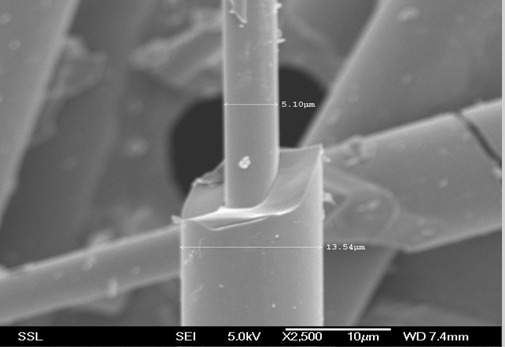
\includegraphics[scale=0.75]{microwire.jpg}
  \caption{Elektronimikroskooppikuva lasip��llysteisest� mikrolankaelektrodista. L�hde: http://www.jyi.org/research/re.php?id=1493}
  \label{fig:microwire}
 \end{center}
\end{figure}


\subsection{Piipohjaiset implantit}

Piipohjaiset implantit valmistetaan elektroniikasta ja MEMS-teknologiasta tutuilla menetelmill�. Kyseisill� tekniikoilla saadaan aikaan tarkkoja, eritt�in pieni� rakenteita, joiden s�hk�iset ominaisuudet ovat hyvin hallittavissa. Kuvassa \ref{fig:silicon_probe} n�kyy perinteisen muotoinen piipiikkielektrodi, johon on my�s lis�tty kemiallinen sensori.

\begin{figure}[htcb]
 \begin{center}
  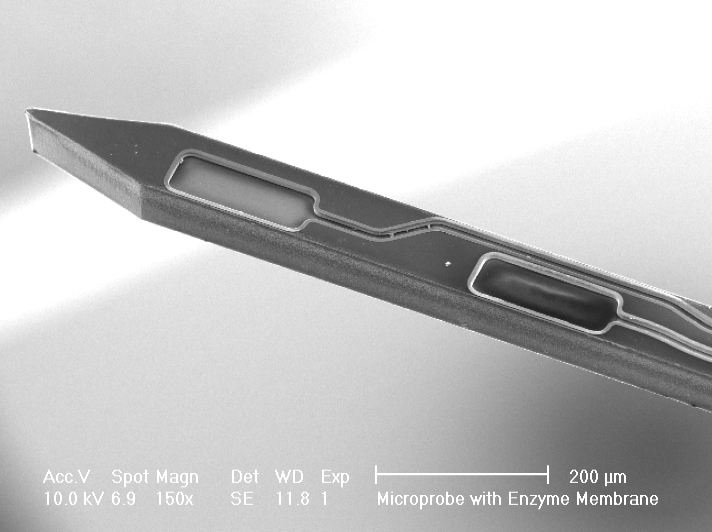
\includegraphics[scale=0.5]{silicon_probe.jpg}
  \caption{Elektronimikroskooppikuva piipohjaisesta elektrodista, joka sis�lt�� my�s kemiallisen sensorin. L�hde: http://samlab.epfl.ch/page-15473-en.html}
  \label{fig:silicon_probe}
 \end{center}
\end{figure}

Pii-implantit valmistetaan usein siten, ett� yhdess� elementiss� on monta yksitt�ist� elektrodia oman tukivartensa p��ss� joko jono- tai matriisimuodostelmassa (kuva \ref{fig:silicon_array}). Nykyisill� menetelmill� kunkin piikin korkeus on yksil�llisesti valittavissa ja yhdess� piikiss� voi olla useita mittauspisteit�, joten neuroverkkojen 3D-mittaukset ovat mahdollisia.

Piipohjaisia valmistusmenetelmi� k�ytett�ess� voi itse implantin materiaalina olla my�s jokin muu kuin pii, kuten polymeeri tai metalli. Valmistusmenetelm�t kuitenkin rajoittavat materiaalivalikoimaa jonkin verran.

\begin{figure}[htcb]
 \begin{center}
  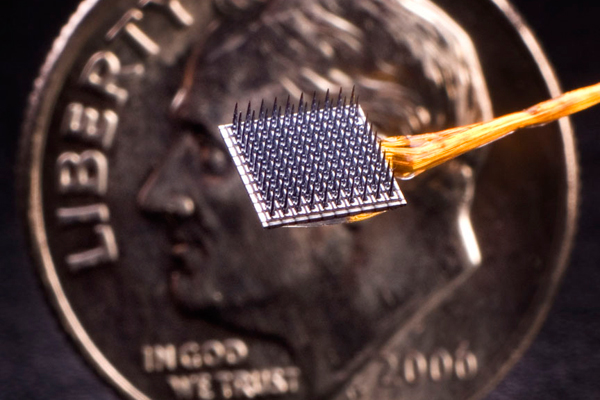
\includegraphics[scale=0.5]{silicon_array.jpg}
  \caption{Piielektrodimatriisi. L�hde: http://www.newscientist.com/blogs/ shortsharpscience/2011/03/power-of-thought-neural-implan.html}
  \label{fig:silicon_array}
 \end{center}
\end{figure}

\subsection{Polymeeri-implantit}

Polymeereja on tutkittu implanttimateriaaleina jonkin verran. Niiden ehdottomana etuna on elastisuuden tuoma parempi kimmoyhteensopivuus kudoksen kanssa, mutta heikkoutena implantoinnin vaikeus: joustavaa implanttia ei voi ty�nt�� suoraan aivokalvon l�pi, vaan v�yl� t�ytyy puhkaista erikseen. T�m� on sek� haastavampaa ett� aiheuttaa enemm�n tuhoa kudoksessa kuin pii- ja mikrolankaimplanttien tapauksessa. \cite{Polikov}

%\clearpage
\section{Implantointi ja keskushermoston immuunivaste}

Implantoinnin ja elektrodien itsens� aiheuttama immuunivaste aivoissa on suurin elektrodin toimintaa haittaava tekij�. Siisp� elektrodien suorituskyvyn maksimoimiseksi on t�rke�� ymm�rt�� ne biologiset mekanismit, jotka ajavat immuuniprosessia.

On huomattava, ett� neuronit muodostavat vain alle 25\% aivokudoksesta; loput ovat verenkiertoon liittyvi� soluja sek� gliosyyttej�, hermotukisoluja, jotka ovat aivojen immuunivasteen merkitt�vimm�t osallistujat. N�ist� astrosyytit muodostavat matriksia (arpikudosta) vauriokohtaan ja mikrogliasolut toimivat sytotoksisina soluina tai fagosyyttein� tuhoten vaurioitunutta kudosta.

Implantointiprosessi on usein v�kivaltainen - neulamaiset elektrodit ty�nnet��n aivokudoksen l�pi kohteeseensa, mik� rikkoo hiussuonia,  aivojen tukikudosta ja solurakenteita. Lis�ksi implantti syrj�ytt�� tielt��n kudosta aiheuttaen painetta implantin v�litt�m�ss� l�heisyydess� olevassa kudoksessa. T�m� mekaaninen vaurio aiheuttaa keskushermostolle ominaisen vasteen, joka muistuttaa paljon muiden kudosten paranemisprosessia. Mainittakoon, ett� vauriokohtaan kertyy nestett� aiheuttaen turvotusta, mik� edelleen pahentaa kudokseen kohdistuvaa painetta.\cite{Polikov}

Paranemisprosessi on tehokas, ja implantointireitin vauriot yleens� korjautuvat joidenkin viikkojen aikana. Varsinaisena ongelmana onkin, ett� implantti jota mikrogliasolut eiv�t saa tuhottua saa aikaan kroonisen vierasesinevasteen, jossa mikrogliasolut eritt�v�t jatkuvasti proteolyyttisi� entsyymej� tuhoten samalla ymp�r�iv�� hermokudosta \cite{McConnell} ja astrosyytit muodostavat implantin ymp�rille arpikudosta. T�m� reaktio tulee esille vasta varsinaisen immuunireaktion j�lkeen ja on suurin syyllinen ep�onnistuneisiin implantointeihin. Kuvaavaa on, ett� er��ss� tutkimuksessa 25\%:ssa implantoiduista piielektrodeista oli merkkej� aktivoituneista mikrogliasoluista viel� 6 kuukautta implantoinnin j�lkeen. \cite{Schmidt} Yleisesti ottaen jo kuudessa viikossa arpikudos saattaa olla niin paksu, ett� se haittaa pysyv�sti elektrodin toimintaa. \cite{Turner}

\subsection{Implantointimenetelm�n vaikutus}

Tutkimukset osoittavat, ett� veren seerumilla on merkitt�v� osuus arpeutumisen edist�misess� ja veri my�s aiheuttaa tulehdusreaktion kudoksessa. T�m�n takia mit� v�hemm�n verisuonia katkeaa implantoinnin yhteydess�, sit� pienempi on immuunireaktio ja sit� v�hemm�n arpikudosta syntyy. Implantointimenetelm� saattaa vaikuttaa syntyneeseen vaurioon ja siten implantoinnin onnistumiseen, mutta vertailukelpoisia tuloksia ei juuri ole. Eri tutkimusryhm�t ovat kokeilleet eri implantointinopeuksia n. 100 $\mu$m/s ja 8,3 m/s v�lill�, mutta koska tarkasteltava systeemi on niin monimutkainen, on kullakin menetelm�ll� ja nopeudella etunsa ja haittansa. \cite{Polikov}

%Bioaktiiviset pinnat houkuttelevat neuroneita l�helleen ja siten maksimoivat signaalin lyhyell� aikav�lill�, mutta eiv�t hidasta arpikudoksen muodostumista.

%Ongelma: bioaktiivisten aineiden saaminen elektrodille jatkuvalla sy�t�ll�. Mikrofluidistiikka?

\section{Algoritmit}

Kaikkien kuvapohjaisten s��t�systeemien tavoitteena on minimoida erosuure \textbf{e}(t), 
joka tyypillisesti m��ritell��n 

\begin{equation}
\textbf{e}(t) = \textbf{s}(\textbf{m}(t), \textbf{a}) - \textbf{s}^* .
\label{eq:e}
\end{equation}

T�m� yleinen muoto kattaa l�hes kaikki s��t�algoritmit: \textbf{m} on 
kuvasta tehdyist� mittauksista muodostettu vektori ja \textbf{a} puolestaan sis�lt�� 
mahdollisen a priori -tiedon systeemist�, kuten kameran ominaisuuksia tai n�k�kent�ss� 
olevien kappaleiden 3D-malleja. N�ist� lasketaan \textbf{s}, joka on joukko kuvan 
visuaalisia ominaisuuksia. Kameran ja/tai s��dett�v�n kappaleen haluttuun paikkaan ja 
asentoon liittyv�t visuaaliset ominaisuudet muodostavat $\textbf{s}^*$:n, jolloin 
\textbf{e} saadaan laskettua. $\textbf{s}^*$ voi olla staattinen tai ajan funktio.
Eri s��t�\-algo\-ritmit eroavat toisistaan l�hinn� siin� suhteessa, miten \textbf{s} on 
valittu.~\cite{Chaumette_2006}

\subsection{Kuvapohjainen s��t�}

Kuvapohjaisessa s��d�ss� tarkasteltavana suureena on suoraan kuvasta saatu informaatio,
kuten tiettyjen objektien kuvakoordinaatit; tarkemmin ottaen kolmiulotteisessa avaruudessa
olevien pisteiden koordinaattien projektio kuvatasolle. K�ytt�m�ll� hyv�ksi kameran 
tiedettyj� ominaisuuksia, kuten polttov�li� ja dimensioiden suhdetta, 2D-koordinaateista 
voidaan estimoida objektin 3D-paikka. Kuitenkaan t�t� ei yleens� tehd�, vaan tyydyt��n 
k�ytt�m��n $\textbf{s}^*$:n� joukkoa ennaltam��r�ttyj� pisteiden paikkoja kuvatasolla.

S��d�n tuloksena on kameran reitti, joka kulkee pienint� virhett� kohti jokaisessa pisteess�.
Seurauksena on se, ett� reitti ei ole v�ltt�m�tt� suora eik� tasanopeuksinen, mutta 
kuitenkin joka tilanteesta (paitsi joissain tapauksissa $\pi$ radiaanin kierrosta)
on yksiselitteinen suunta tiedossa.

\subsection{Paikkapohjainen s��t�}

Paikkapohjaisessa s��d�ss� kuvan ominaisuuksista ensin arvioidaan kameran ja/tai 
objektin paikka ja orientaatio ulkopuolisessa koordinaatistossa, joiden perusteella 
muodostetaan erosuure. Paikka\-pohjainen s��t� perustuu siis aina estimaatioon ja on 
siten tietyiss� sovelluksissa kuvapohjaista ep�vakaampi.
T�m� s��t�algoritmi tarvitsee toimiakseen a priori -tietoa ymp�rist�st��n, kuten kameran 
parametrit ja tarkasteltavan objektin 3D-mallin, jotta havainnoista voidaan laskea edell�mainitut
asiat.

Paikkapohjaista s��t�� k�ytett�ess� on luonnollista, ett� s��d�n tuloksena kameran liikkeet
ovat suoria, vaikka kuva v�lill� n�enn�isesti menisikin huonompaan suuntaan. Oleellista on,
ett� ne objektit, joista asento ja paikka arvioidaan, pysyv�t kuvassa jatkuvasti, mik� 
t�ll� s��t�algoritmilla ei aina toteudu. Sit� onkin korjattu esim. lis��m�ll� virheeseen termi, 
joka sakottaa liian l�helle kuvan reunaa joutuvasta objektista.

\subsection{Syvyysn�k�}

Syvyysn�k� voidaan toteuttaa monella tapaa, ja monesti se helpottaa visual servo 
-k�ytt�� poistamalla (ainakin suurelta osin) ep�varmuuden kuvan syvyysparametrien
arvioinnista.

Ihmiselle luonnollisin tapa toteuttaa syvyysn�k� on kahdella kameralla, ns. stereon�k�.
Kun tiedet��n kameroiden v�linen et�isyys, voidaan kummankin kameran kuvassa n�kyvien 
objektien et�isyys laskea kolmiomittaamalla. Erityisesti kuvapohjaista s��t�� on 
luonnollista laajentaa stereokamerasysteemiksi, t�ll�in on vain otettava huomioon se,
ett� kummallakin kuvalla on oma suhteensa todelliseen maailmaan.

Toinen tapa toteuttaa er��nlainen stereon�k� on ottaa samalla kameralla uusi kuva
m��ritellyn liikkeen j�lkeen. T�ll� ei saavuteta samoja reaaliaikaetuja kuin kahden
kameran j�rjestelm�ss�, mutta toisaalta kuvia voi ottaa eri suunnista ja eri 
et�isyyksilt�, kunnes tarkkuus on toivottu.

Jos toimintaymp�rist� on kontrolloitu, sen 3D-malli voi olla kuvan\-k�sittely\-tieto\-koneen
muistissa, jolloin er��nlainen syvyysn�k� on mahdollinen: kuvasta voidaan p��tell�
mitk� mallin piirteist� ovat n�kyviss� ja polttov�lin sek� piirteiden suhteellisen koon
perusteella m��ritt�� et�isyys piirteisiin.

\subsection{Hahmontunnistus}

Hahmontunnistuksessa kuvainformaatiosta yritet��n poimia esiin erilaisia piirteit�, joita
voidaan luokitella ja n�inollen saada kone ``ymm�rt�m��n'' n�kem�ns� kuva. T�llaisia
piirteit� voi olla esimerkiksi kuvassa olevat ihmiset, tietty esine joka robotin tulee
paikallistaa tai mahdolliset tiell� olevat esteet. Sen lis�ksi ett� kuvasta voidaan
tunnistaa kohteita, niiden liikett� voidaan my�s seurata tai estimoida muutamien kuvien
perusteella. T�ss� kappaleessa tutustutaan muutamaan perusk�sitteeseen ja menetelm��n,
jotka liittyv�t hahmontunnistukseen.

\subsubsection{Segmentointi}

Erilaisten hahmontunnistusmenetelmien perustana on yleens� kuvan segmentointi, eli
jakaminen osiin erilaisten ominaisuuksien perusteella. Segmentoinnin p��m��r�n� on jakaa
kuva pienempiin osiin siten, ett� yksitt�isten osien sis�lt�m�ll� kuvainformaatiolla on
jotakin yhteist�. Yksitt�iseen osaan kuuluvilla pikseleill� voi olla esimerkiksi
samantapainen v�ri, kirkkaus tai tekstuuri. Segmentointia k�ytet��n yleens�
konen�k�sovelluksissa prosessoinnin alkuvaiheessa. Segmentoidusta kuvasta voidaan edelleen
tunnistaa tarkemmin kiinnostavia kohteita kehittyneemmill� menetelmill�.

Segmentointi voidaan suorittaa erilaisilla menetelmill� sovelluksen tarpeiden mukaan.
Yksinkertaisin menetelm� on kuvan kynnyst�minen kirkkauden tai tietyn v�rikomponentin
mukaan. Kynnystyksell� tarkoitetaan kuvan pikseleiden jakamista yleens� kahteen osaan sen
mukaan, onko kyseisen pikselin arvo suurempi vai pienempi kuin asetettu kynnysarvo.
Kynnystykseen perustuvissa menetelmiss� asetetulla kynnysarvolla on eritt�in suuri
merkitys lopputulokseen. Liian suuri kynnysarvo aiheuttaa sen, ett� haluttuja piirteit� ei
saada esiin kuvasta, ja vastaavasti liian pieni kynnysarvo sekoittaa halutut piirteet ei
haluttuihin piirteisiin. Kynnystys on toimiva menetelm� yksinkertaisissa kuvissa, joissa
halutut kohteet erottuvat selke�sti taustasta.

Hieman kehittyneemmiss� menetelmiss� yritet��n muodostaa yhten�isist� piirteist� koostuvia
alueita. Er�s t�llainen algoritmi on K-means~\cite{Alsabti_1998}. K-means algoritmi on
perusmuodossaan seuraavanlainen:
\begin{enumerate}
	\label{lst:k-means}
	\item Valitse joukko alueiden keskipisteit�pisteit� (esim. satunnaisesti)
	\item Liit� jokainen kuvan piste siihen alueeseen, joka minimoi varianssin kyseisen
				pisteen ja alueen keskipisteen v�lill� \label{lst:k-means_assign}
	\item Laske alueiden keskipisteet uudelleen
	\item Mik�li alueiden keskipisteet muuttuivat edellisess� kohdassa, palaa
				kohtaan~\ref{lst:k-means_assign}
\end{enumerate}
Algoritmin kohdassa~\ref{lst:k-means_assign} varianssilla tarkoitetaan suuretta, joka voi
riippua pikseleiden v�rist�, kirkkaudesta, tekstuurista ja sijainnista. N�it�
ominaisuuksia voidaan painottaa erilaisilla kertoimilla.

Erilaisia reunantunnistusmenetelmi� on tutkittu ja kehitetty paljon, ja niill� saavutetaan
hyvi� tuloksia. Reunat jakavat kuvan yleens� melko hyvin yhten�isiksi alueksi, joten
reunantunnistusalgoritmeja voidaan k�ytt�� joko sellaisenaan kuvan segmentoimiseen tai
jonkun muun menetelm�n pohjana. Reunantunnistuksessa reunoihin tulee yleens� pieni�
aukkoja kohtiin, joissa kuuluisi olla reuna. On kuitenkin olemassa algoritmeja, jotka
pystyv�t tunnistamaan ja t�ytt�m��n t�llaiset aukot~\cite{Pathegama_2004}.

\subsubsection{Mallinnesovitus}

Hahmontunnistusta voidaan suorittaa etsim�ll� kuvasta kohteita, jotka vastaavat jotakin
toista kuvaa. T�t� kutsutaan mallinnesovitukseksi~(engl.~template matching). Kuvasta
voidaan siis etsi� esimerkiksi tietyn henkil�n kasvoja yritt�m�ll� sovittaa siihen
mallinnekuvaa kyseisist� kasvoista. Sovittamisessa mallinnekuvaa liu'utetaan tutkittavan
kuvan p��ll�. Mik�li mallinnekuva sopii johonkin kohtaan kuvaa riitt�v�n hyvin, on hahmo
tunnistettu kyseisest� kohdasta. Mallinnekuvaa joudutaan yleens� py�ritt�m��n ja sen kokoa
muuttamaan, jotta mallinne sopisi kuvaan. T�m� on laskennallisesti eritt�in raskasta.

Mallinnesovituksessa voidaan hy�dynt�� kuvan segmentoimista. T�ll�in mallinnetta voidaan
yritt�� ainakin ensiksi sovittaa vain tiettyihin kuvan osiin, jotka ovat tietyn
muotoisia, v�risi� tai tietyss� paikassa. T�m� saattaa suotuisassa tilanteessa nopeuttaa
mallinnesovitusta huomattavasti.



\section{Sovellukset}


\section{Yhteenveto}

\begin{frame}[t]
\frametitle{Yhteenveto}
\vspace{0.5cm}

\begin{itemize}
  \item N�in
  \item Noin
  \item Nuin
\end{itemize}

\end{frame}

%% L�hdeluettelo
\clearpage
\addcontentsline{toc}{section}{Viitteet}
\bibliographystyle{unsrt_fin}
\bibliography{visualservo_references}

\end{document}
